\section{Laborversuch Proben des Verdauungssystems}

\subsection{Menschlicher Magen}
\begin{figure}[h!]
    \centering
    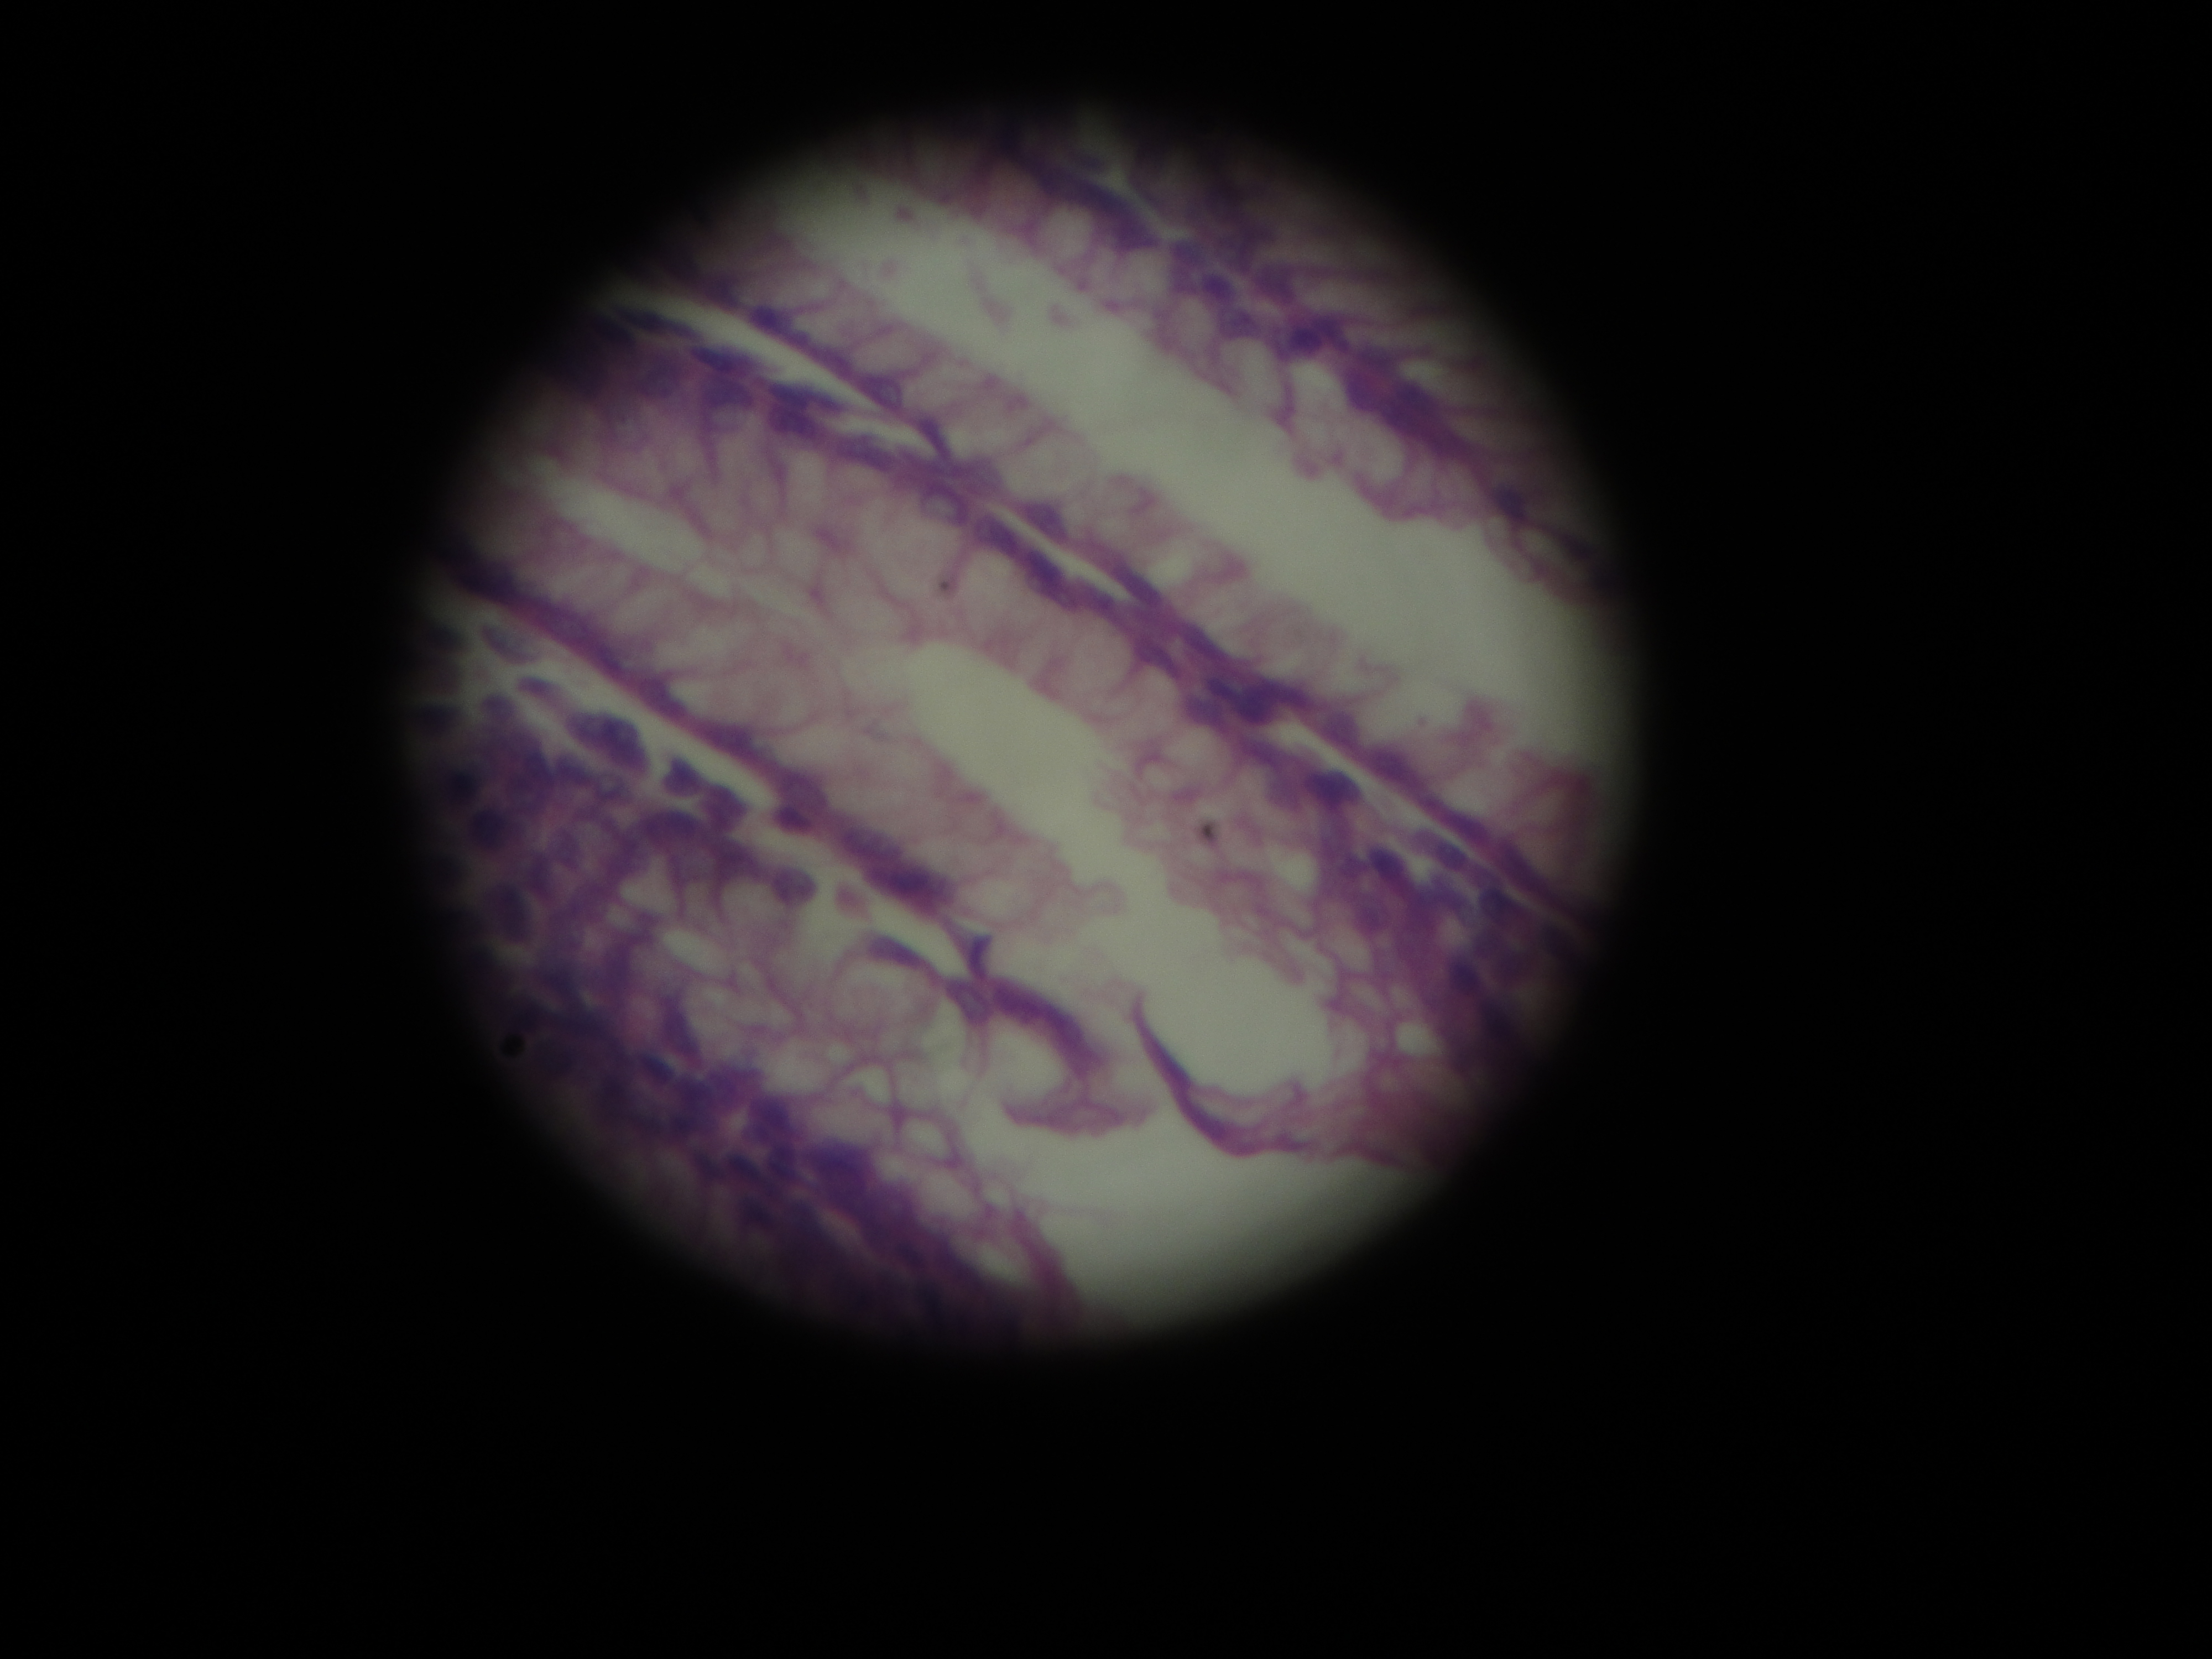
\includegraphics[width=0.5\textwidth]{fig/digestion/DSC02784.JPG}
    \caption{Menschlicher Magen}
    \label{fig:human_stomach}
\end{figure}

\subsection{Menschliche Leber}
\begin{figure}[h!]
    \centering
    \includegraphics[width=0.5\textwidth]{fig/digestion/DSC02790.JPG}
    \caption{Menschliche Leber}
    \label{fig:human_liver}
\end{figure}
\clearpage

\subsection{Menschliche Bauchspeicheldrüse}
\begin{figure}[h!]
    \centering
    \includegraphics[width=0.5\textwidth]{fig/digestion/DSC02790.JPG}
    \caption{Menschliche Bauchspeicheldrüse}
    \label{fig:human_pancreas}
\end{figure}
\begin{figure}[h!]
    \centering
    \includegraphics[width=0.5\textwidth]{fig/digestion/DSC02794.JPG}
    \caption{Menschliche Bauchspeicheldrüse (Inselapparat)}
    \label{fig:human_pancreas_2}
\end{figure}
\clearpage

\subsection{Menschlicher Dünndarm}
\begin{figure}[h!]
    \centering
    \includegraphics[width=0.5\textwidth]{fig/digestion/DSC02792.JPG}
    \caption{Menschlicher Dünndarm}
    \label{fig:human_mamal_lieum}
\end{figure}

